\newpage
\section{Summary}
\begin{description}
	\item \textbf{What?}
	   \begin{itemize}
		   \item Bayesian data analysis is a flexible method to fit any type of statistical model. 
			 \item Maximum likelihood is actually a special case of Bayesian model fitting.
	   \end{itemize}
	\item \textbf{Why?}
			\begin{itemize}
				\item Makes it possible to define highly customizable models.
				\item Makes it possible to include information from many sources, such as data and expert knowledge.
				\item Quantifies and retains the uncertainty in parameter estimates and predictions.
			\end{itemize}
	\item \textbf{How?}
	\begin{itemize}
	       \item R! Using ABC, MCMCpack, JAGS, STAN, R-inla, Python, etc.
	       \end{itemize}
\end{description}

%---------------------------------------------------------------------------------------
% ---------- Appendix A-----------------------------------------------------------------
%---------------------------------------------------------------------------------------
\appendix

%---------------------------------------------------------------------------------------
% ---------- Appendix B-----------------------------------------------------------------
%---------------------------------------------------------------------------------------
\section*{Exercises -- Solutions}
\begin{itemize}
	
\item \textbf{Exercise }\ref{ex1.4.1}:  
$$ P(L|Y) = \frac{P(Y|L) P(L)}{P(Y)}$$
Note that $$P(Y) = P(Y,L) + P(Y,\overline{L}) = P(Y|L) P(L) + P(Y|\overline{L}) P(\overline{L}),$$ so 
$$P(L|Y) =\frac{(.55)(.52)}{(.55)(.52)+(.85)(.48)} = 0.41.$$

\item \textbf{Exercise }\ref{ex1.4.2}: 
\begin{description}
\item[Step 1:] assign events to $A$ or $X$. You want to know what a woman's probability of having cancer is, given a positive mammogram. For this problem, actually having cancer is $A$ and a positive test result is $X$.
\item[Step 2:] list out the parts of the equation (this makes it easier to work the actual equation):
$$P(A) = 0.01, P(\overline{A})= 0.99, P(X|A)=0.9, P(X|\overline{A}).$$ 
\item[Step 3:] insert the parts into the equation and solve. Note that as this is a medical test we have
$$\frac{0.9\cdot 0.01}{(0.9)(0.01)+(0.08)(0.99)} = 0.10.$$ 
The probability of a woman having cancer, given a positive test result, is thus 10\%. 
\end{description}


\newpage\noindent\item \textbf{Exercise }\ref{ex3.5.1}
\begin{enumerate}
	\item To justify a prior, we might say that our strength of fairness is equivalent to having previously seen the coin flipped 100 times and coming up heads in 50\% of those flips. Hence the prior would be $\text{Beta}(\theta|50,50)$ (this is not the only correct answer, of course; you might instead be more confident, and use, say,  $\text{Beta}(\theta|500,500)$ if you suppose you've previously seen 1,000 flips with 50\% heads).\newl 
	The posterior is then $\text{Beta}(\theta|50+9,50+1)$, which has a mean of $\frac{59}{59+51} = 0.536$. This is the predicted probability of heads for the next (11th) flip.
\item In this case, we use a $\text{Beta}(\theta|0.5,0.5)$ prior, like the one used in Example\ref{Ex:unusualprior}, because it expresses a belief that the coin is either head-biased or tail-biased. \newl The posterior is  $\text{Beta}(\theta|0.5+9,0.5+1)$, which has a mean of $\frac{9.5}{9.5+1.5} = 0.863$. This is the predicted probability of heads for the next (11th) flip. Notice that it is quite different than the conclusion from Part 1.
\end{enumerate}


\item \textbf{Exercise }\ref{ex4.2.1} \\
The commands 
\begin{quote}
\small \texttt{> post = BernBeta(c(1,1),  \\ 
\ \ \ \ \ \ \ \  c(rep(1,40),rep(0,10)))}\\
\texttt{> post = BernBeta(c(1,1),    \\
\ \ \ \ \ \ \ \   c(rep(1,15),rep(0,35)))} \normalsize
\end{quote}
yield the display below.
\begin{center}
		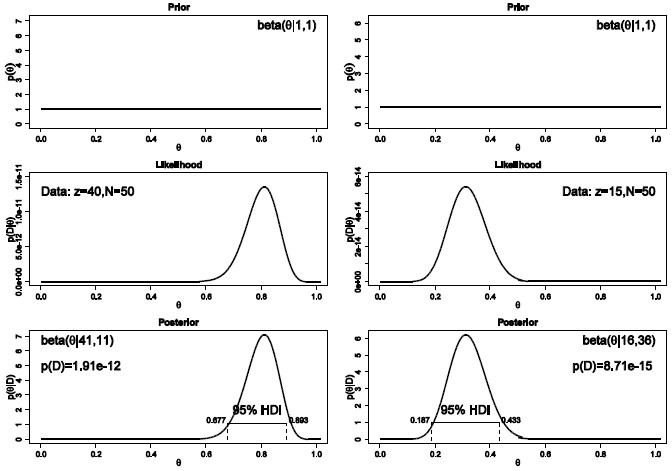
\includegraphics[width=\linewidth]{Images/exsection4.png}
\end{center}
In both cases, the 95\% HDI excludes $\theta=0.5$, and so we conclude that people are indeed biased in their responses, toward $F$ in the first case and toward $J$ in the second case. 
\end{itemize}